\newpage
\part{User Service Node}
\newpage
\chapter{Web Application}
\label{ch:5}

\section{Introduction}
In this chapter, the proposed user service node model will be thoroughly examined---from the perspective of the web application; along with the development objectives in mind to achieve the desired performance and acceptable user experience.


\section{Development Objectives}
Among the development objectives stated in chapter~\ref{ch:1}, two in particular can be classified to be related to the user service node and one will be the main focus in this chapter: Graphical User Interface. The graphical user interface can be dissected into multiple sub-objectives as follows:
\begin{enumerate}
    \item User Interface (UI) Design.
    
            \vspace{-1.5mm}
            \textbf{Objective:} Create an intuitive and user-friendly interface that allows users to easily navigate through the app.
            
            \vspace{-1.5mm}
            \textbf{Details}:
            \begin{itemize}
                \vspace{-1mm}
                \item Develop a dashboard for quick access to main features.
                \vspace{-1mm}
                \item Design task creation and map editing interfaces with drag-and-drop functionality.
                \vspace{-1mm}
                \item Ensure responsive design for compatibility with various devices.
            \end{itemize}

%%%%%%%%%%%%%%%
            
    \item Task Management System.

        \vspace{-1.5mm}
        \textbf{Objective}: Develop a robust task management system for creating, scheduling, and monitoring tasks.

        \vspace{-1.5mm}
        \textbf{Details}:
        \begin{itemize}
            \vspace{-1mm}
            \item Allow users to create, edit, and delete tasks.
            \vspace{-1mm}
            \item Enable task scheduling.
            \vspace{-1mm}
            \item Assign Task to a robot easily.
        \end{itemize}

%%%%%%%%%

    \item Reliable data storage and management.
    
        \vspace{-1.5mm}
        \textbf{Objective}: Implement a reliable data storage solution for tasks, maps, and user data.

        \vspace{-1.5mm}
        \textbf{Details}:
        \begin{itemize}
            \vspace{-1mm}
            \item Use a relational database (e.g., MYSQL) for structured data storage.
            \vspace{-1mm}
            \item Save data like tasks and maps in JSON files for easy access and modification.
            \vspace{-1mm}
            \item Ensure data integrity and implement backup and recovery mechanisms.
            \vspace{-1mm}
            \item Implement data encryption for sensitive information.
        \end{itemize}

%%%%%%%%%
    
    \item Map Creation and Management.
    
        \vspace{-1.5mm}
        \textbf{Objective}: Provide tools for users to create and manage maps for robot navigation.

        \vspace{-1.5mm}
        \textbf{Details}:
        \begin{itemize}
            \vspace{-1mm}
            \item Implement a map editor with features for drawing and editing paths, obstacles, and waypoints.
            \vspace{-1mm}
            \item Allow users to save and load maps.
            \vspace{-1mm}
            \item Integrate map data with the robot's navigation system for real-time updates.
        \end{itemize}
%%%%%%%%%

    \item Real-Time Control and Monitoring
        
        \vspace{-1.5mm}
        \textbf{Objective}: Enable real-time control and monitoring of the robot.

        \vspace{-1.5mm}
        \textbf{Details}:
        \begin{itemize}
            \vspace{-1mm}
            \item Implement controls for manual operation of the robot.
            \vspace{-1mm}
            \item Display real-time data such as status, motors' speed and position.
        \end{itemize}

%%%%%%%%%

    \item Integration with Robot’s API
        
        \vspace{-1.5mm}
        \textbf{Objective}: Ensure seamless integration with the robot’s API for command execution and data retrieval.

        \vspace{-1.5mm}
        \textbf{Details}:
        \begin{itemize}
            \vspace{-1mm}
            \item Implement API endpoints for sending commands to the robot.
            \vspace{-1mm}
            \item Retrieve and display various data from the robot.
            \vspace{-1mm}
            \item Handle API error responses and provide appropriate user feedback.
        \end{itemize}

%%%%%%%%%
\newpage
    \item Python API Development
        
        \vspace{-1.5mm}
        \textbf{Objective}: Develop a Python-based API for enhanced functionality and interoperability.

        \vspace{-1.5mm}
        \textbf{Details}:
        \begin{itemize}
            \vspace{-1mm}
            \item Design and implement a Python API for additional command execution and data retrieval.
            %\newpage
            \vspace{-1mm}
            \item Utilize web sockets for real-time communication and updates between the client and server.
            \vspace{-1mm}
            \item Ensure the Python API integrates seamlessly with the existing system.
            \vspace{-1mm}
            \item Provide detailed documentation and examples for using the Python API.
        \end{itemize}

%%%%%%%%%

    \item Performance Optimization
        
        \vspace{-1.5mm}
        \textbf{Objective}: Optimize the web app for performance and scalability.

        \vspace{-1.5mm}
        \textbf{Details}:
        \begin{itemize}
            \vspace{-1mm}
            \item Use efficient algorithms for task scheduling and map processing.
            \vspace{-1mm}
            \item Implement caching strategies to reduce load times.
        \end{itemize}
\end{enumerate}


%%%%%%%%%%%%%%%%%%%%%%%%%%%%%%%%%%5
\section{Used Tools and Frameworks} % + state reason behind using them
A comprehensive robot control system is implemented using a combination of front-end  and back-end  technologies. The front-end \footnote{Full code implementation can be viewed at: \url{https://github.com/meh-land/web\_App}} is developed with React.js and TypeScript, utilizing libraries such as React Router DOM, Axios, React Flow, and various hooks (\texttt{useState}, \texttt{useContext}, and \texttt{useEffect}). The back end is built with Laravel\footnote{Full code implementation can be viewed at: \url{https://shorturl.at/VdtOP}, \url{https://shorturl.at/6a0cM}}, while Python scripts are executed to perform specific tasks. This document details the frameworks and libraries used, the reasons behind their selection, and their roles in the overall system.

\subsection{Front-End Implementation}
\subsubsection{A) React.js and TypeScript}

\textbf{React.js} is a popular JavaScript library for building user interfaces, particularly single-page applications (SPAs). It allows developers to create reusable UI components, making the development process more efficient and manageable \cite{reactjs}. 
\newpage
\textbf{TypeScript} is a superset of JavaScript that adds static type definitions, enabling developers to catch errors early in the development process and improve code maintainability and readability \cite{reactTS}.


\begin{itemize}
    \item \textbf{Create a new React.js project}:
    \begin{verbatim}
    npx create-react-app my-app
    \end{verbatim}

    \vspace{-4.5mm}
    
    \item \textbf{Create a new React.js project with TypeScript}:
    \begin{verbatim}
    npx create-react-app my-app --template typescript
    \end{verbatim}

    \vspace{-4.5mm}
    
    \item \textbf{Navigate to the project directory}:
    \begin{verbatim}
    cd my-app
    \end{verbatim}
    
    \vspace{-4.5mm}
    
    \item \textbf{Start the development server}:
    \begin{verbatim}
    npm start
    \end{verbatim}
\end{itemize}

\vspace{-10mm}

\subsubsection*{B) React Router DOM}
\vspace{-3mm}
\textbf{React Router DOM} is a routing library for React that enables the creation of dynamic and complex navigation structures in web applications. It manages the navigation between different components and pages in the application \cite{reactrouter}\cite{reactrouterdom}.
\vspace{-2mm}
\begin{itemize}
    \item \textbf{Usage}: It allows the robot control system to have multiple views, such as robots, maps, tasks, and dashboard, while maintaining a seamless user experience. It ensures that users can easily switch between various functionalities of the robot control system. To install React Router DOM, you can use the following npm command \cite{reactrouterdom}:
    \vspace{-1mm}
    \begin{verbatim}
    npm install react-router-dom
    \end{verbatim}

    \vspace{-6mm}
    
    Once React Router DOM have been installed, import the needed components for the demo inside App.js/.tsx. Then add the following code snippets:

    \lstinputlisting[language=JavaScript, style=CodeStyleJavaScript, caption= React Router Dom Implementation (1), label=cd:socket.io-client, firstline=1, lastline=10]{CodeSnippets/ReactRouterDom.tsx}
    \newpage
    \lstinputlisting[language=JavaScript, style=CodeStyleJavaScript, caption= React Router Dom Implementation (2), label=cd:socket.io-client2, firstline=11, lastline=24]{CodeSnippets/ReactRouterDom.tsx}
    
\end{itemize}

\vspace{-5mm}

\subsubsection*{C) Axios}

\textbf{Axios} is a promise-based HTTP client for making requests to external APIs or back-end services. It simplifies the process of sending asynchronous HTTP requests and handling responses \cite{axios}.
\vspace{-2mm}
\begin{itemize}
    \item \textbf{Usage}: Axios is used for communication between the front-end React application and the back-end Laravel server. It handles tasks such as fetching real-time robot data, sending control commands, and retrieving analytics information.To install axios, you can use the following
npm command:
        \begin{verbatim}
    npm install axios
    \end{verbatim}
    \vspace{-3mm}
    Once you have installed Axios, it can be used as follows:
    \vspace{1mm}
    \lstinputlisting[language=JavaScript, style=CodeStyleJavaScript, caption= Axios get request Implementation (1), label=cd:axios, firstline=1, lastline=15]{CodeSnippets/axios.tsx}
    \newpage
    \lstinputlisting[language=JavaScript, style=CodeStyleJavaScript, caption= Axios get request Implementation (2), label=cd:axios2, firstline=16, lastline=42]{CodeSnippets/axios.tsx}
\end{itemize}

\subsubsection*{D) socket.io-client}

\textbf{socket.io-client} package is a library that enables real-time, bidirectional, and event-based communication between the client and server. It is particularly useful for applications that require instant updates, such as real-time notifications \cite{socketio-client} \cite{socketio-react}.
\vspace{-2mm}
\begin{itemize}
    \item \textbf{Usage}: socket.io-client package is used to enable real-time updates by listening for changes in logs, status and Motors' speed from the server, and if there is change, new data is displayed.\footnote{Full code implementation can be viewed at: \url{https://github.com/meh-land/web\_App}}
    To install socket.io-client package, you can use the following npm command:
        \begin{verbatim}
    npm install socket.io-client
    \end{verbatim}
    Once you have installed the Socket.IO client library, you can initialize the client as follows:

    \vspace{-2mm}
\begin{enumerate}
    \item \textbf{Import the \texttt{io} function from the \texttt{socket.io-client} package}:
\lstinputlisting[language=JavaScript, style=CodeStyleJavaScript, caption= Import the io function from the socket.io-client package, label=cd:socket.io-client, firstline=2, lastline=2]{CodeSnippets/socket.io-client.tsx}
    \vspace{-3mm}
    This imports the \texttt{io} function from the \texttt{socket.io-client} package, which is used to establish a connection with the Socket.IO server.

    \item \textbf{Initialize the socket connection}:
\lstinputlisting[language=JavaScript, style=CodeStyleJavaScript, caption= Initialize the socket connection, label=cd:socket.io-client, firstline=5, lastline=9]{CodeSnippets/socket.io-client.tsx}
    \vspace{-3mm}
    If the front-end and server are served from the same domain, the default \texttt{io()} initialization is sufficient. If they are served from different domains, you need to provide the server URL.

    \item \textbf{Initiate connection and listen for events}:
\lstinputlisting[language=JavaScript, style=CodeStyleJavaScript, caption= Initiate connection and listen for events, label=cd:socket.io-client, firstline=12, lastline=18]{CodeSnippets/socket.io-client.tsx}
\vspace{-2mm}
    Here, we set up a listener for the \texttt{file\_changed\_logs} event. When this event is received, the \texttt{data} is used to update the \texttt{logs} state and is also logged to the console.
\newpage
    \item \textbf{Cleanup on component unmount}:
\lstinputlisting[language=JavaScript, style=CodeStyleJavaScript, caption= Cleanup on component unmount, label=cd:socket.io-client, firstline=22, lastline=25]{CodeSnippets/socket.io-client.tsx}
    This ensures that the \texttt{file\_changed\_logs} event listener is removed when the component is unmounted, preventing potential memory leaks.
\end{enumerate}

By following these steps, you can effectively manage real-time updates in your application using the Socket.IO client library.

\textbf{Using Flask and Socket.IO for Real-Time File Monitoring} \footnote{Full code implementation can be viewed at: \url{https://shorturl.at/M1oNT}}

The following steps demonstrate how to use Flask and Socket.IO to monitor file changes in real-time and notify clients of updates.

\begin{enumerate}
    \item \textbf{Import the necessary libraries}:

    \lstinputlisting[language=Python, style=CodeStylePython, caption= Import the necessary libraries, label=cd:socket.io-client, firstline=1, lastline=6]{CodeSnippets/socketAPI.py}

    \vspace{-2mm}
    
    These imports bring in the necessary libraries for creating a Flask application, handling real-time communication with Socket.IO, and monitoring file changes with watchdog.

    \item \textbf{Initialize the Flask app and Socket.IO}:
    \lstinputlisting[language=python, style=CodeStylePython, caption= Initialize the Flask application and sets up Socket.IO with cross-origin support.
    , label=cd:socket.io-client, firstline=8, lastline=9]{CodeSnippets/socketAPI.py}
\newpage
    \item \textbf{Function to monitor file changes}:
    \vspace{2mm}
    \lstinputlisting[language=python, style=CodeStylePython, caption= Function to monitor file changes.
    , label=cd:socket.io-client, firstline=44, lastline=54]{CodeSnippets/socketAPI.py}

    \item \textbf{Run the Flask application with Socket.IO}:
    \vspace{2mm}
    \lstinputlisting[language=python, style=CodeStylePython, caption= Run the Flask application with Socket.IO.
    , label=cd:socket.io-client, firstline=60, lastline=67]{CodeSnippets/socketAPI.py}
    \vspace{-2mm}
        Creates and starts threads to monitor each file and runs the Flask application with Socket.IO in debug mode.

    % Hello there
    % It seems you are busy, just wanted to say hi
    % Good job you did here

    % Thanks ^^

\end{enumerate}


\end{itemize}

% In the appendix, you can find more details regarding code usage (see Appendix~\ref{webapp}).

\subsubsection*{E) React Flow}
\vspace{-2mm}
\textbf{React Flow} is a library for building node-based graphical interfaces. It provides tools to create interactive flow diagrams, which are essential for visualizing complex systems and processes \cite{reactflow} \cite{reactflow-examples}.

\begin{itemize}
    \item \textbf{Usage}: React Flow is utilized to design and visualize the path of the robot. It allows users to create, modify, and monitor the robot's movement through an intuitive graphical interface. To install reactflow, you can use the following
npm command:

\vspace{-2mm}
            \begin{verbatim}
    npm install reactflow
    \end{verbatim}
    %\vspace{-3mm}
    \newpage
    Once you have installed reactflow, you can use it as follows:
\vspace{2mm}
    \lstinputlisting[language=python, style=CodeStylePython, caption= React Flow Implementation.
    , label=cd:socket.io-client, firstline=1, lastline=37]{CodeSnippets/reactflow.tsx}
\end{itemize}

\newpage

\subsubsection*{F) React Hooks}

React hooks are functions that let developers use state and other React features without writing a class \cite{react-hooks-intro} \cite{react-hooks-reference}. The primary hooks used in this project include:

\begin{itemize}
    \item \texttt{useState}: Manages state within functional components \cite{react-hooks-state}.
    \item \texttt{useContext}: Shares state and data across components without prop drilling \cite{react-usecontext}.
    \item \texttt{useEffect}: Handles side effects such as data fetching and updating the DOM \cite{react-hooks-effect}.

\end{itemize}

The hooks mentioned above are employed to manage the application's state, handle data fetching, update the user interface in response to state changes, and share data between components efficiently.


\subsection{Back-End Implementation}
\subsubsection*{A) Laravel}

\textbf{Laravel} is a PHP framework designed for web application development. It follows the Model-View-Controller (MVC) architectural pattern, providing a robust structure for building scalable and maintainable back-end systems \cite{laravel-docs}.
\vspace{-2mm}
\begin{itemize}
    \item \textbf{Usage}: Laravel serves as the back-end framework for the robot control system. It handles user authentication, data storage, and communication with the front end. The framework's built-in features, such as routing, middleware, Passport, and caching, streamline the development process and ensure a secure and efficient server-side operation.

    % In the appendix, you can find more details on our website (see Appendix~\ref{webapp}).
    \vspace{-2mm}
    \begin{itemize}
        \item \textbf{Middleware}: Middleware in Laravel acts as a filtering mechanism for HTTP requests entering your application. It ensures that only authenticated and authorized users can access specific routes and resources \cite{laravel-middleware}.
        \begin{enumerate}
            \item  To create middleware, use the following command:
        \begin{verbatim}
        php artisan make:middleware MiddlewareName
        \end{verbatim}
\vspace{-4mm}
        \item  Middleware in Laravel acts as a filtering mechanism for HTTP requests entering your application. It ensures that only authenticated users can access specific routes and resources.

\newpage
        \lstinputlisting[language=php, style=CodeStylePHP, caption= Middleware usage to protect routes in a Laravel application..
    , label=cd:socket.io-client, firstline=1, lastline=3]{CodeSnippets/middleware.php}

        \end{enumerate}

        
        \item \textbf{Passport}: Laravel Passport provides a full OAuth2 server implementation for Laravel applications. It is used for API authentication, allowing the robot control system to securely authenticate users and manage tokens \cite{laravel-passport}. To install Passport, use the following commands:
        \begin{verbatim}
        composer require laravel/passport
        php artisan passport:install
        \end{verbatim}

 \vspace{-4mm}
        
        \item \textbf{File Writing}: Laravel provides a robust file storage system that supports local file storage. This is used to store necessary data required by the robot control system \cite{laravel-filesystem}. 
        
        When using the local driver, all file operations are relative to the root directory defined in your filesystems configuration file. By default, this value is set to the storage/app directory. Therefore, the following method would write to storage/app/example.txt:
        \vspace{1mm}
        \lstinputlisting[language=php, style=CodeStylePHP, caption= Writing data to file in storage/app in laravel project.
    , label=cd:socket.io-client, firstline=1, lastline=3]{CodeSnippets/filewriting.php}
 
    \end{itemize}
\end{itemize}


\subsubsection*{B) Python API (Flask)}

\textbf{Flask} is a micro web framework written in Python. It is designed to be simple and flexible, allowing developers to build web applications quickly and with minimal overhead. Flask provides the essentials needed to get a web server up and running but leaves many decisions about architecture and additional features up to the developer. This makes it a popular choice for both small applications and large-scale projects \cite{flask-quickstart}.

\begin{itemize}
\item \textbf{Usage}: Flask in this code serves as the foundation for creating a web server that can handle HTTP requests and integrate with SocketIO for real-time communication. It provides the necessary infrastructure to serve web pages and handle client connections, while the SocketIO integration allows for dynamic updates based on file changes detected by the watchdog observers. 


\newpage
\item \textbf{Commands}:
    \begin{itemize}
        \item \textbf{Install Flask and Flask-SocketIO}:
        \begin{verbatim}
        pip install flask flask-socketio
        \end{verbatim}
        \vspace{-2mm}
        \item \textbf{Install Watchdog} (for file system monitoring):
        \begin{verbatim}
        pip install watchdog
        \end{verbatim}
        

    \end{itemize}

\end{itemize}

\vspace{-3mm}

\subsubsection*{C) ROS (rospy) Scripts}

\textbf{Python} is a versatile programming language known for its simplicity and extensive library support. It is widely used in robotics for tasks such as data processing, machine learning, and control algorithms. In this context, \textbf{rospy} is the Python client library for ROS (Robot Operating System), which facilitates communication and coordination between various components in a robotic system.

\begin{itemize}
\item \textbf{Usage}: rospy scripts are executed within the Laravel framework to perform specific tasks that require complex computations or interactions with the robot hardware. These tasks include syncing tasks, and executing control algorithms to operate the robot. rospy scripts leverage ROS topics, services, and actions to communicate with the robot and control its behavior in real-time.
\end{itemize}


The combination of React.js, TypeScript, React Router DOM, Axios, React Flow, and React hooks on the front end, along with Laravel and Python scripts on the back end, provides a powerful and efficient architecture for the robot control system. Each framework and library was chosen for its specific strengths and capabilities, ensuring a robust, maintainable, and scalable solution for managing and controlling the robot. This comprehensive setup enables the development of an intuitive user interface, efficient data handling, and seamless integration with the robot hardware, making it an ideal choice for this graduation project.


\section{Design and Development Strategy}

The Robot Control System Web Application is designed to provide an intuitive and efficient interface for controlling and monitoring robots in various environments. This project aims to leverage modern web technologies to create a versatile platform that can be accessed from any device with internet connectivity.
\newpage
\subsection{System Architecture}
\vspace{-1.5mm}
The system architecture follows the Model-View-Controller (MVC) concept to ensure a clear separation of concerns and maintainability.
\vspace{-3mm}
\subsubsection{A) Client-Side Application}
\vspace{-2.5mm}
The client-side application is developed using React.js, a popular JavaScript library for building user interfaces. The application will feature a responsive design to ensure it functions well on both desktop and mobile devices. Key components include:
\vspace{-1mm}
\begin{itemize}
    \item \textbf{View (UI Components)}:
    \begin{itemize}
    \vspace{-1mm}
        \item \textbf{Dashboard}: A central hub displaying the status and controls for connected robots.
        \vspace{-1mm}
        \item \textbf{Control Panel}: An interface for sending commands to the robots, including movement, actions, and other functions.
        \vspace{-1mm}
        \item \textbf{Maps Creation}: A feature to create maps/paths for robots to follow.
        \vspace{-1mm}
        \item \textbf{Tasks Management}: A feature to assign, monitor, and manage tasks for the robots.
    \end{itemize}
\end{itemize}
\vspace{-3mm}
\subsubsection{B) Server-Side Application}
\vspace{-2.5mm}
The server-side application will handle communication between the client-side application and the robots, manage user authentication, and store data. Key components include:
\vspace{-2mm}
\begin{itemize}
    \item \textbf{Controller}:
    \begin{itemize}
    \vspace{-1mm}
        \item \textbf{REST API}: Endpoints for retrieving and updating robot data, user information, and application settings.
        \vspace{-1mm}
        \item \textbf{Business Logic}: Processing commands from the client-side application and executing corresponding actions.
    \end{itemize}
    \vspace{-1mm}
    \item \textbf{Model}:
    \vspace{-1mm}
    \begin{itemize}
        \item \textbf{Database}: A MySQL database for storing persistent data such as user profiles, robot configurations, maps, and tasks.
    \end{itemize}
\end{itemize}

\subsubsection{C) Robot Control Integration}
\vspace{-2.5mm}
The Robot Control Integration ensures seamless communication and control between the web application and the physical robots.  Key components include:

\begin{itemize}
\vspace{-1mm}
    \item \textbf{Command Execution (Controller)}: The control units receive commands from the server-side application's REST API and execute movement and action instructions sent from the client-side application.
    \vspace{-1mm}
    \item \textbf{Real-Time Feedback (Model)}: The control units send real-time data from sensors and motors back to the server-side application. This data is stored in the database and used to update the client-side application's Dashboard and other interfaces.
    \vspace{-1mm}
    \item \textbf{Connectivity (View)}: The control units maintain a reliable and secure connection to the server-side application via Wi-Fi or other wireless protocols, ensuring continuous operation and efficient communication.
\end{itemize}

By adhering to the MVC architecture, the system ensures a structured and scalable approach to development, enhancing maintainability and ease of integration.
%%%%%%%%%%%%%%%%%%%%%%%%%%
\subsection{User Interface Design}
\vspace{-1.5mm}
The user interface (UI) design will prioritize ease of use, clarity, and accessibility. It will follow a modular design approach, with reusable components for different parts of the application.
\vspace{-1.5mm}
% In the appendix, you can find more details on our website (see Appendix~\ref{webapp}).

\subsubsection{A) Dashboard}
\vspace{-1mm}
The dashboard will provide an overview of connected robot, displaying its current status, location, and speed. Users can quickly select a robot to view more detailed information or take control.
\vspace{-1mm}
\subsubsection{B) Control Panel}
\vspace{-1mm}
The control panel will offer an intuitive layout for sending commands to the selected robot.
\vspace{-5mm}
\subsubsection{C) Maps Creation}
\vspace{-1mm}
Tools for creating and managing maps or paths that robots can follow. This includes the ability to define way points, set navigation routes, and visualize the paths in a user-friendly manner.
\newpage
\subsubsection{D) Tasks Management}
\vspace{-1mm}
 Functionality for creating, scheduling, and assigning tasks to robots. This includes setting task priorities, monitoring task progress, and receiving notifications upon task completion or failure.
\vspace{-1mm}
\subsection{Implementation Plan}
The implementation of the Robot Control System Web Application follows an iterative development process, with key milestones including:
\begin{enumerate}
    \item \textbf{Requirements Gathering}: Define detailed requirements and use cases for the application.
    \item \textbf{Design Phase}: Create mockups, and a detailed system architecture.
    \item \textbf{Development Phase}: Implement the client-side and server-side applications, followed by integration with the robot control units.
    \item \textbf{Testing Phase}: Conduct thorough testing to ensure functionality, performance, and security.

\end{enumerate}


%%%%%%%%%%%%%%%%%%%%%%%%%%%%%%%%%%%%%%%%

\section{Output} % + state which of the listed specs were fulfilled here
\subsection{Home Page}
The dashboard for managing robots, featuring sections for Robots, Maps, and Tasks. The sidebar allows users to navigate to different sections including Home, Robots, Maps, and Tasks. Figure \ref{fig:homePage} shows how the home page is presented.

\begin{figure}[h!]
    \centering
    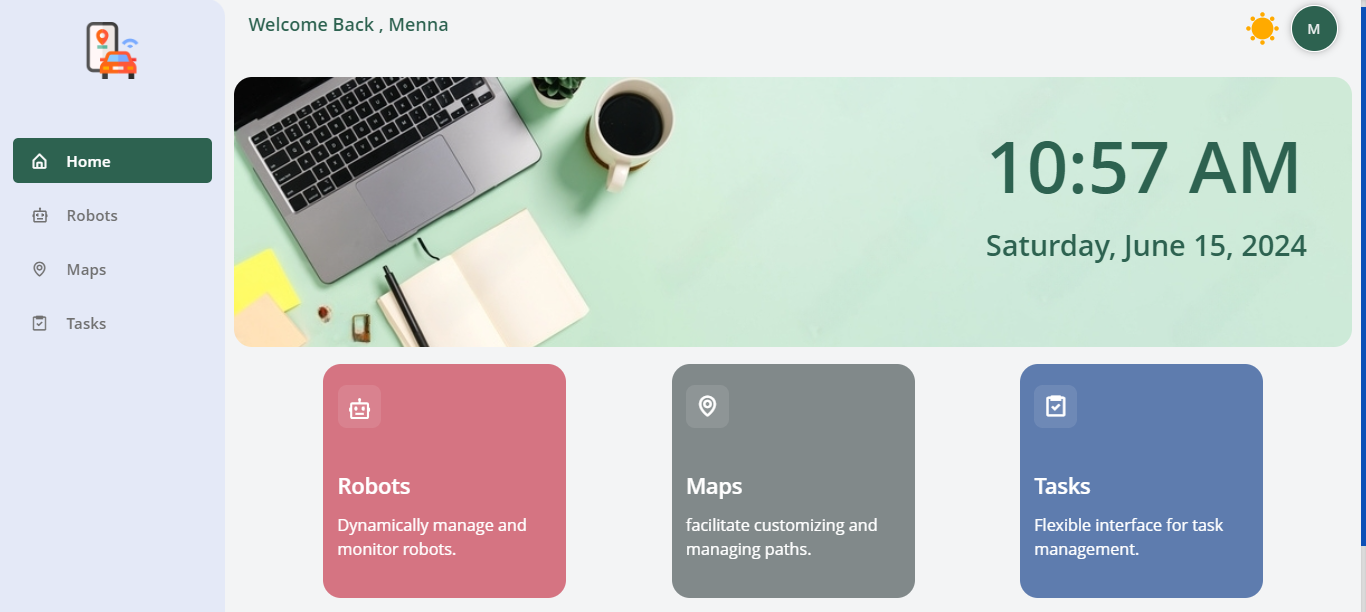
\includegraphics[scale=0.35]{Figures/WebApp/HomePage.png}
    \caption{Home page}
    \label{fig:homePage}
\end{figure}
\newpage
\subsection{Robots Management}

    The robots management dashboard---shown in figure \ref{fig:robots-dashboard}---provides a comprehensive view of all robots. It includes a table displaying the robots and offers options to add new robots, edit existing robot details, or delete robots from the system.

    \begin{figure}[h!]
        \centering
        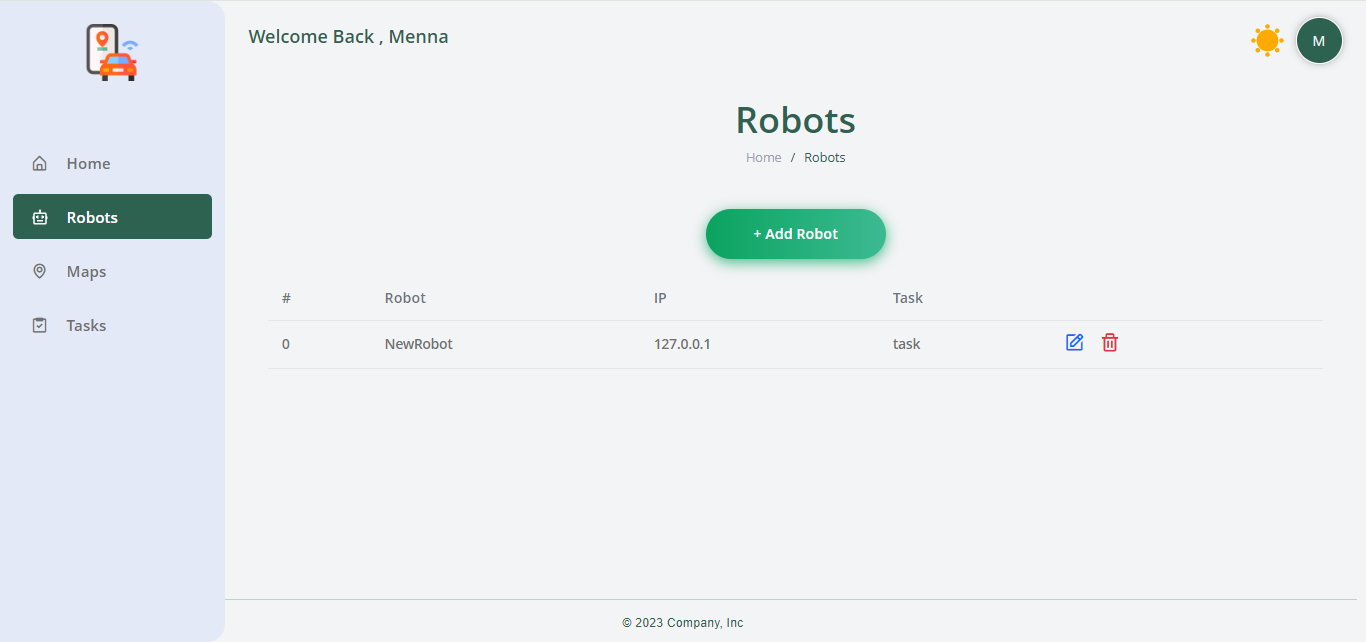
\includegraphics[scale=0.31]{Figures/WebApp/Robots.png}
        \caption{Robots management dashboard}
        \label{fig:robots-dashboard}
    \end{figure}


    Figure \ref{fig:create-robot} shows a popup form used for adding new robots to the management system. Users are prompted to enter the robot's name and IP address.

    \begin{figure}[h!]
        \centering
        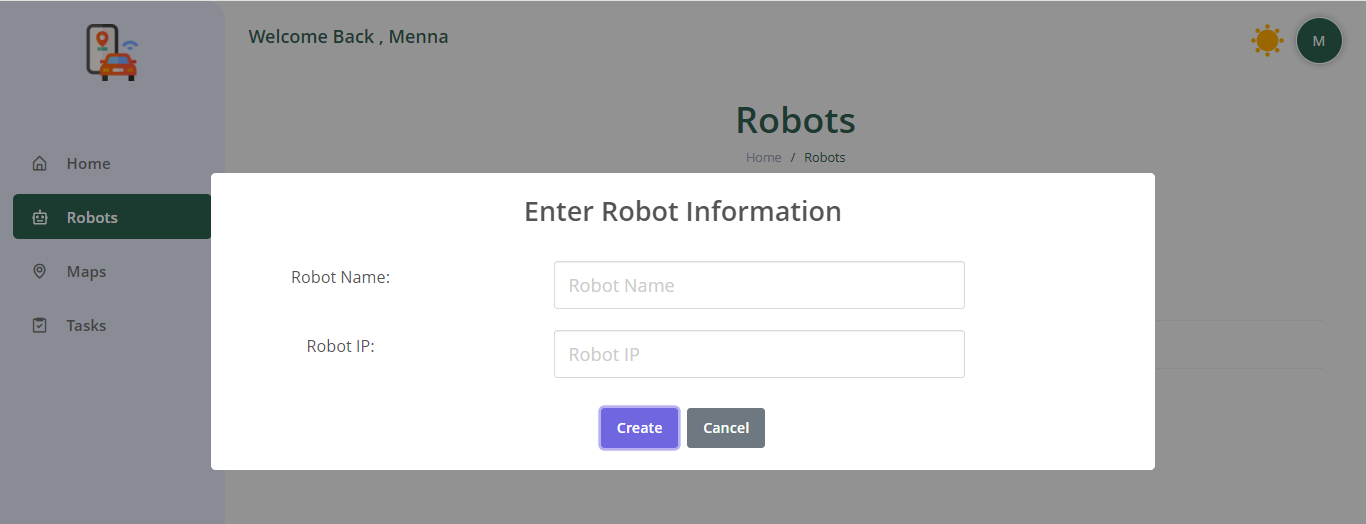
\includegraphics[scale=0.31]{Figures/WebApp/createRobot.png}
        \caption{Creating new robot}
        \label{fig:create-robot}
    \end{figure}

    Figure \ref{fig:edit-robot} shows a popup form used for editing the information of existing robots. Users can update the robot's name, IP address, and assign task to the robot.

    \begin{figure}[h!]
        \centering
        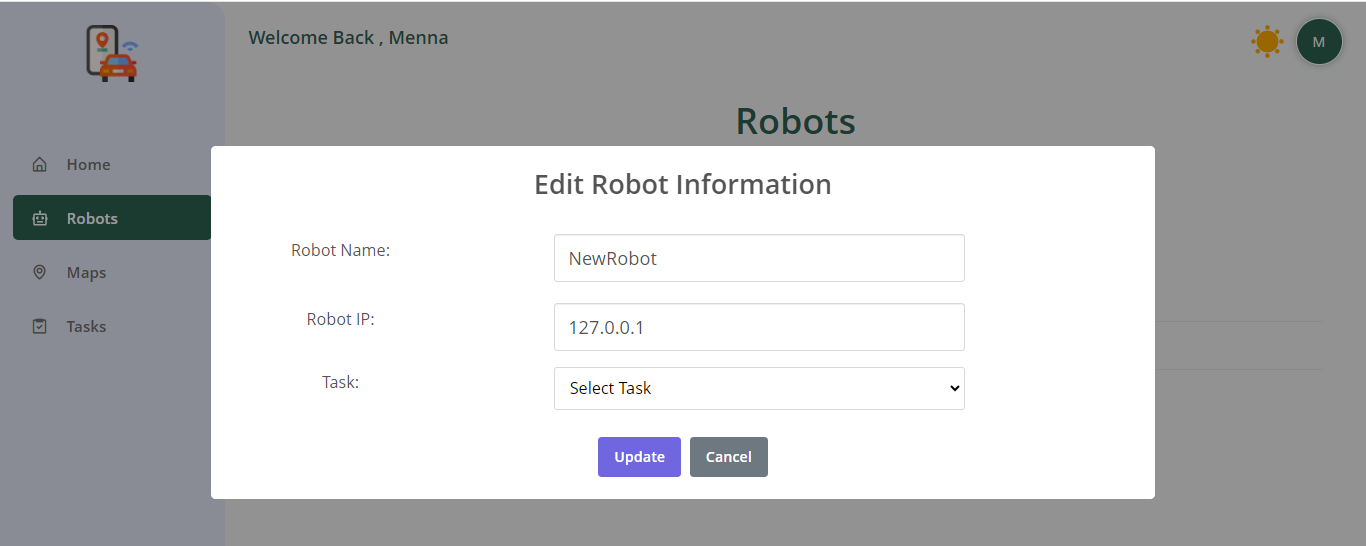
\includegraphics[scale=0.31]{Figures/WebApp/editRobot.png}
        \caption{Editing robot}
        \label{fig:edit-robot}
    \end{figure}

\vspace{-3mm}
\newpage
\subsection{Maps Creation}

    Figure \ref{fig:maps-management} shows the maps management dashboard displays a table listing all maps in the system. It provides options to add new maps or delete existing ones, allowing users to manage their maps efficiently.

    \begin{figure}[h!]
        \centering
        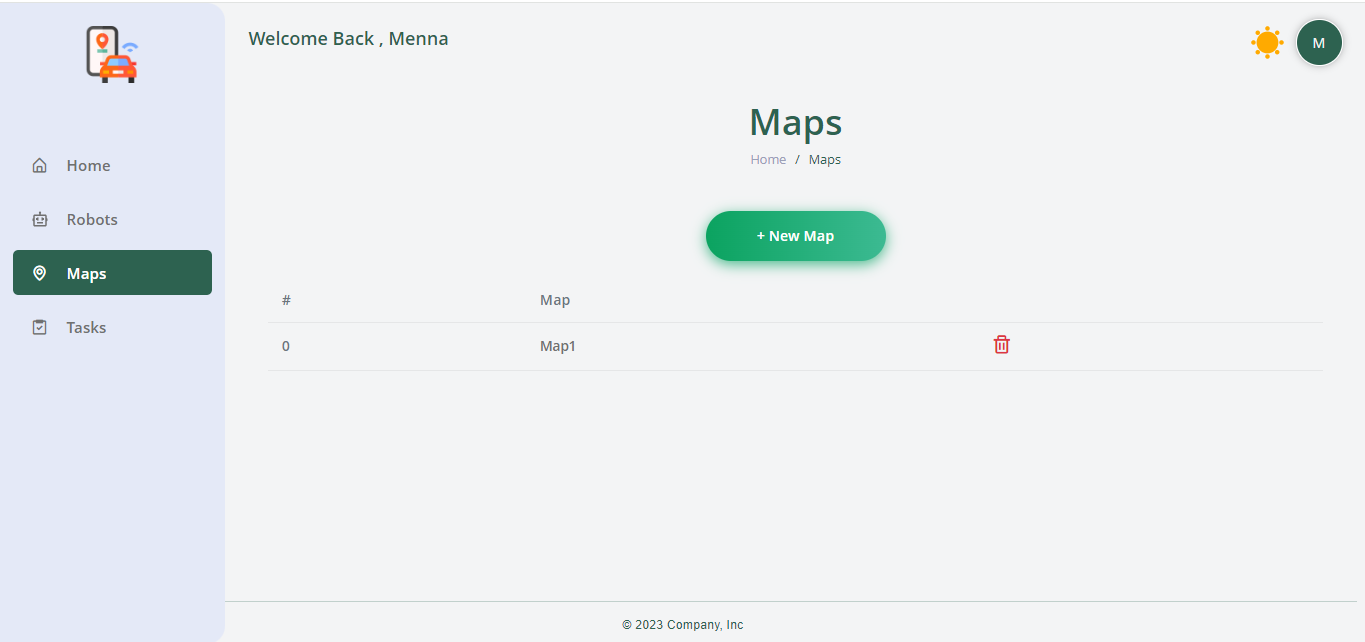
\includegraphics[scale=0.4]{Figures/WebApp/mapsCreation.png}
        \caption{Maps management dashboard}
        \label{fig:maps-management}
    \end{figure}




    The node map editor interface that displays input, default, and output nodes is shown in figure \ref{fig:node-map-editor}. Users can add and name nodes, with guidance on the right side for editing and deleting nodes and connections. This tool facilitates the creation and customization of node maps.

    \begin{figure}[h!]
        \centering
        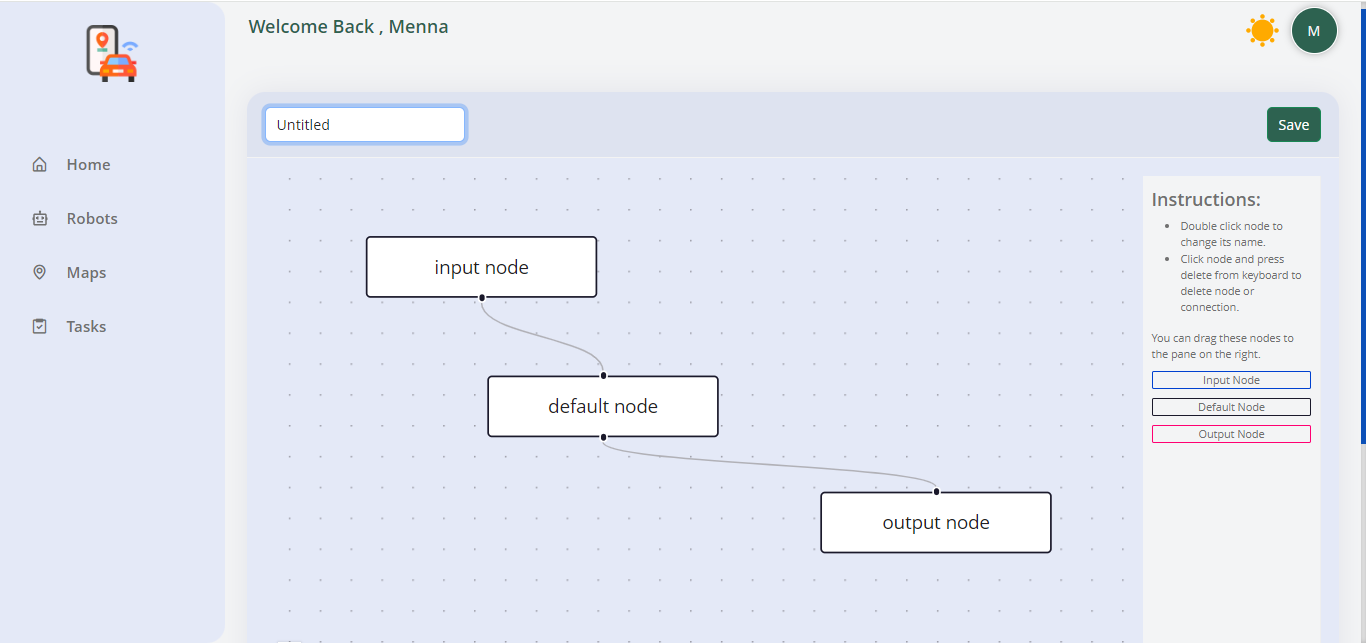
\includegraphics[scale=0.4]{Figures/WebApp/newMap.png}
        \caption{Node map editor}
        \label{fig:node-map-editor}
    \end{figure}

\newpage

    The popup form in the node map editor---shown in figure \ref{fig:edit-node}---allows users to update node information. Users can change the node's label and coordinates, with fields provided for the new label and X and Y coordinates. Options to confirm or cancel the update are included.

    \begin{figure}[h!]
        \centering
        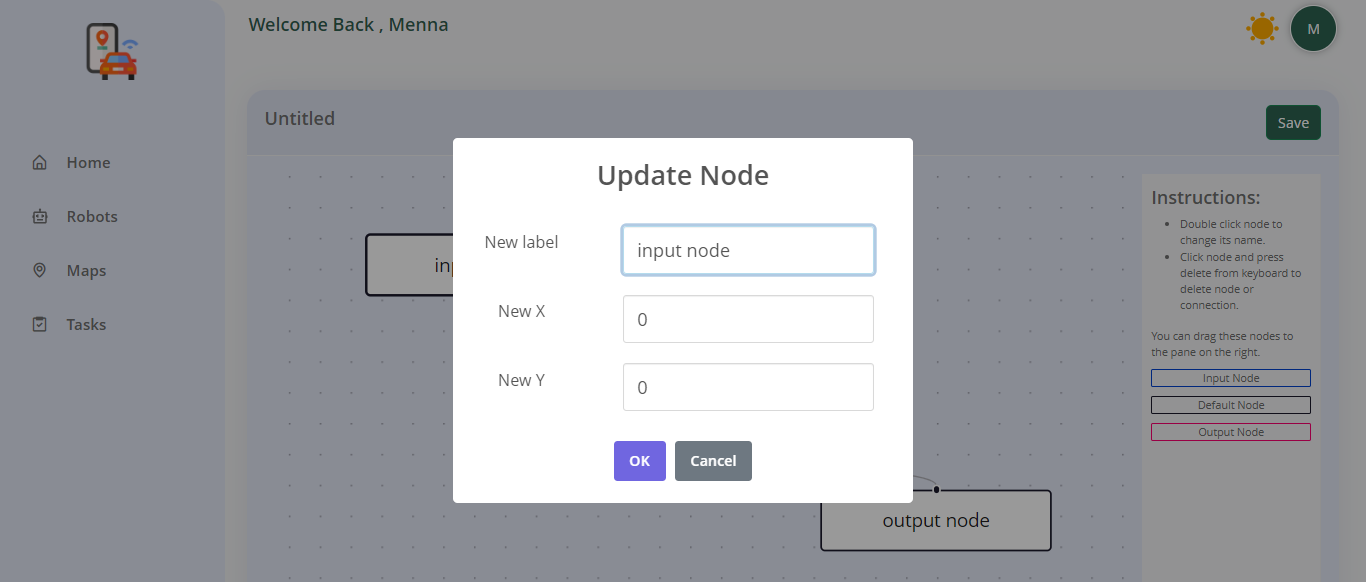
\includegraphics[scale=0.4]{Figures/WebApp/editNode.png}
        \caption{Updating node information.}
        \label{fig:edit-node}
    \end{figure}

    The node map display (figure \ref{fig:edit-map}) showcases a map titled 'Map1' with input, default, and output nodes connected sequentially. The interface provides an 'Edit Map' button, enabling users to modify the map as needed.


    \begin{figure}[h!]
        \centering
        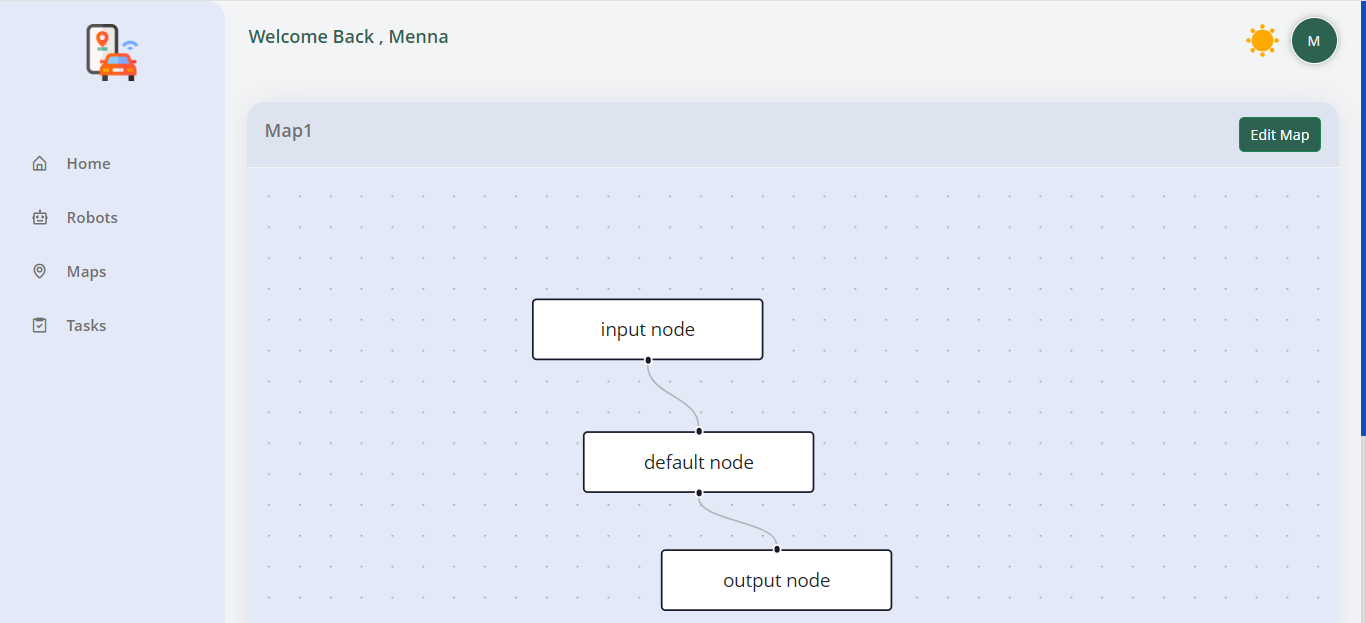
\includegraphics[scale=0.4]{Figures/WebApp/editMap.png}
        \caption{Edit map}
        \label{fig:edit-map}
    \end{figure}

%sup
\newpage

\subsection{Tasks Management}

     The tasks management dashboard (figure \ref{fig:tasks-management}) shows an empty state when no tasks have been added. An illustration and a message prompt users to add new tasks, with a button provided for this purpose.
     \begin{figure}[h!]
        \centering
        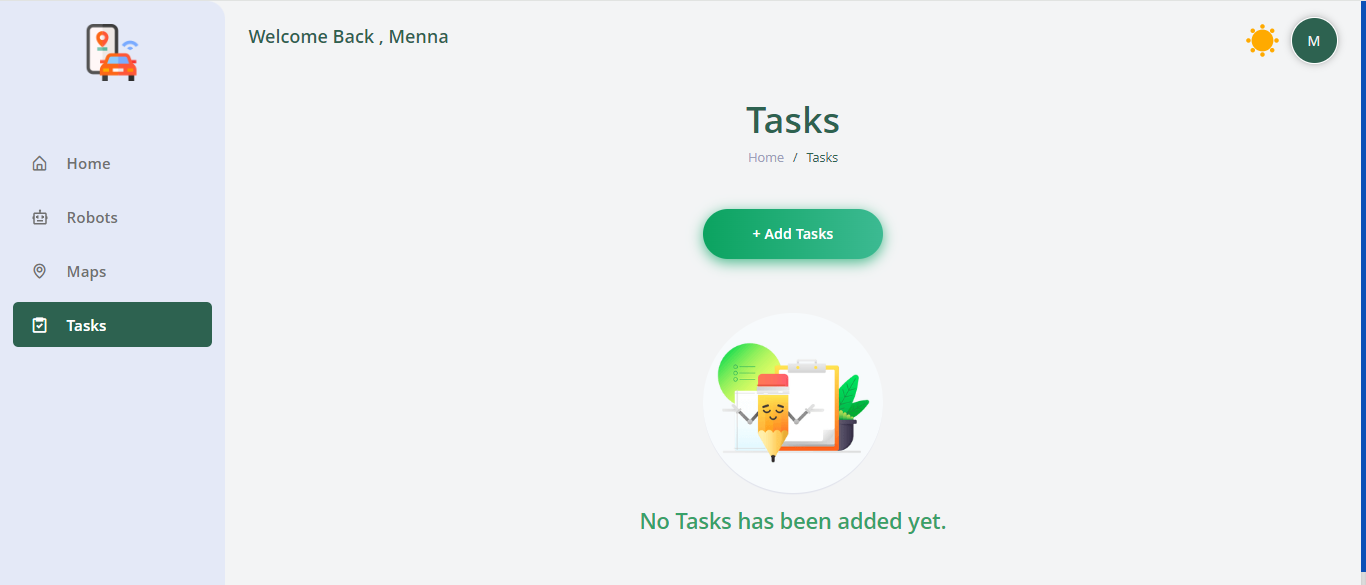
\includegraphics[scale=0.4]{Figures/WebApp/tasks.png}
        \caption{Tasks management dashboard}
        \label{fig:tasks-management}
    \end{figure}

    The popup form in the tasks management dashboard---shown in figure \ref{fig:task-creation}---allows users to enter task information. Users can input details such as the task name, select a map, and specify pick-up and drop-off nodes along with the schedule time. Options to close or save the task are included.
    \begin{figure}[h!]
        \centering
        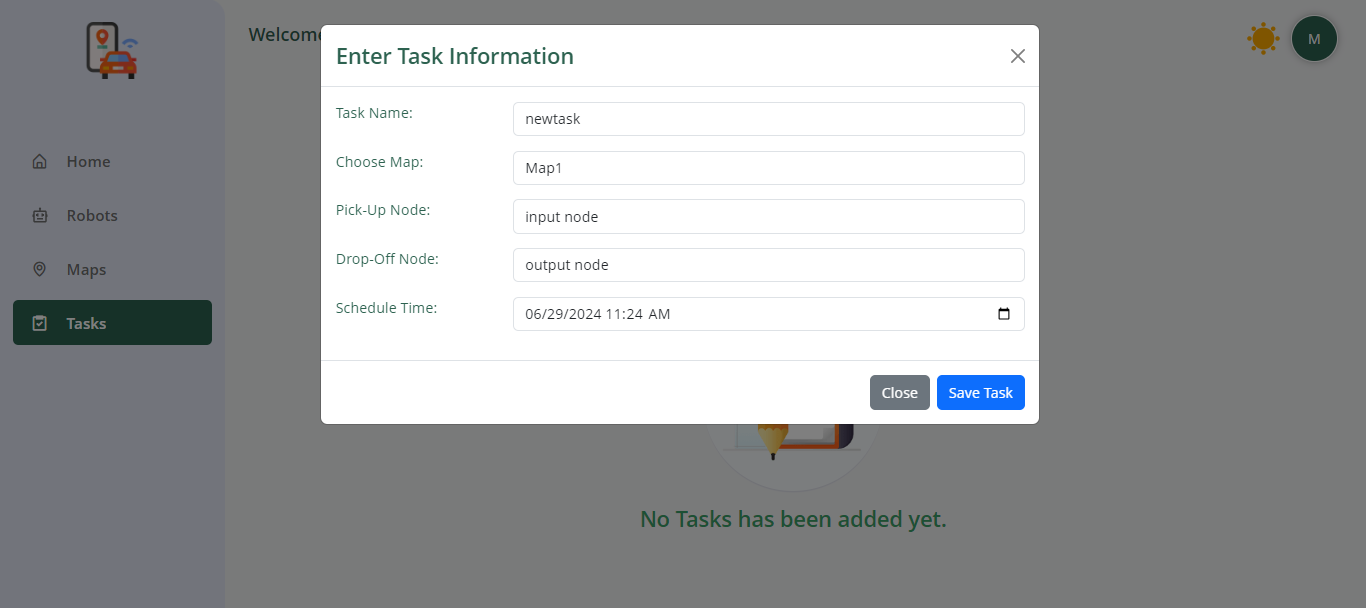
\includegraphics[scale=0.4]{Figures/WebApp/taskCreation.png}
        \caption{New task creation}
        \label{fig:task-creation}
    \end{figure}


%%%%%%%%%%%%%%%%%%%%%%%%%%%%%%%%%%%%%%%%%%%%%%%%%%%%%%%%%%%%%%%%%%%%%%%%%%%%%%%%%

\newpage

\chapter{Server Infrastructure}
In this chapter, the proposed user service node model will be thoroughly examined---from the perspective of the server infrastructure; along with the development objectives in mind to achieve the desired performance and acceptable user experience.

\section{Development Objectives: Overview}
Among the development objectives stated in chapter~\ref{ch:1}, two in particular can be classified to be related to the user service node; one was discussed in chapter~\ref{ch:5} and the other will be the main focus in this chapter: Reliable Server Infrastructure. Making a reliable server infrastructure can be dissected into multiple sub-objectives as follows:
\begin{enumerate}
    \item Creating a reliable server machine on which the web app can run.
    \item Allow this server to communicate with the SBC.
    \item Setup the server such that it has seamless integration withe rest of the network.
\end{enumerate}

% \section{Development Objectives: In-depth View}
% \section{Used Frameworks} % + state reason behind using them
% I think we don't need this particular section in this chapter, it is easier to just talk about the process (Maybe I'll come back to this section later if needed)


\section{System Design}
The server uses Ubuntu 20.04 LTS as its operating system, this is done to offer compatibility with ROS Noetic as mentioned in chapter \ref{ch:CPN-comm}. As it stands, the system does not run any ROS nodes on the server, but it could be useful for future improvements to have a high degree of compatibility between the server and the SBC.

Once the operating system is installed on the server, one must install all the packages required by the web app to operate correctly. Here is only a list of these packages and the utility of each one, the details of installation will be discussed in chapter \ref{ch:res-conc}.
\subsection{Web Application Dependencies}
Here is a list of all the dependencies needed for the correct and reliable operation of the web application. Note that the packages here are mentioned along their version numbers, this is to ensure the reliability of the setup. In other words, these versions are not strictly necessary but these are the only tested versions. Thus they are guaranteed to work coherently.

\begin{itemize}
    \item Apache2: It is the web server of choice.
    \item MySQL: It is the used database.
    \item PHP 8.1: All backend is built using PHP.
    \item Composer: An application-level dependency manager for the PHP programming language that provides a standard format for managing dependencies of PHP software and required libraries.
    \item Laravel 10: The PHP framework used to build the backend.
    \item NPM 8.11: It is the package manager for front-end.
    \item nodejs 16.15: Provides the necessary JavaScript runtime environment and tooling that allows you to effectively use and manage packages through NPM.
\end{itemize}

\subsection{Firewall Configuration}
By default Ubuntu 20.04 uses the Uncomplicated Firewall (UFW)\cite{ubuntu-ufw}, which by default blocks all ports on the host. For the web application to be accessible, UFW needs to be configured in such a way that it allows the appropriate ports. The front-end runs on port 3000 and the back-end runs on port 8000. Thus, ports 3000 and 8000 need to be exposed to the external network. The bash script shown in code snippet \ref{cd:ufw} shows the commands needed to expose the needed ports and refresh UFW in order to make sure that UFW loads the most up-to-date configurations. Note script \ref{cd:ufw} needs sudo privilege to execute correctly.

\lstinputlisting[language=Bash, style=CodeStyleBash, caption=Configure UFW to allow ports, label=cd:ufw]{CodeSnippets/ufwconfig}


% \begin{figure}[h!]
%     \centering
%     
\includegraphics[scale=0.1]{Figures/fool.jpg}
%     \caption{You fell into my trap!}
%     \label{fig:ref1}
% \end{figure}
% \notrickroll

% \lstinputlisting[language=C, style=CodeStyleC, caption=test code, label=cd:haha, firstline=1, lastline=6]{CodeSnippets/haha.c}